% boosting.tex
% Jeremy Barnes, 29/8/1999
% $Id$

% The chapter of my thesis on Boosting
% Still theory

\chapter{AdaBoost and boosting algorithms}
\label{chapter:boosting}

Boosting algorithms (AdaBoost being one of the first) are a very
important recent development in machine learning that has
significantly altered the field.  The name ``Boosting'' is applied to
a range of  machine learning algorithms, all of which combine several
``weak'' hypotheses to form a combined ``strong'' hypothesis that
significantly outperforms all of them.

In this chapter we describe the classic algorithm \emph{AdaBoost}
published by Freund and Schapire in 1996 \cite{Freund96}, and present
results on its properties and generalisation performance.  We then
show that AdaBoost implements the optimisation of a cost functional
via gradient descent, an property that proves to provide a useful
framework for the development of modified algorithms in chapter
\ref{chapter:pboosting}. We digress slightly to look at \emph{normed}
boosting algorithms, a minor modification, and conclude by again
considering the inherent problem of overfitting.

\section{The AdaBoost algorithm}

In essence, the AdaBoost algorithm ``bootstraps'' itself onto another
learning algorithm (the \emph{weak learning algorithm}--the decision
stumps algorithm described in appendix \ref{appendix:stumps} is one
such algorithm), improving its performance by using a ``committee''
(linear combination) of weak hypotheses.

AdaBoost performs \emph{very} well; its combined hypotheses generally
perform significantly better than \emph{any} non-boosted algorithm
(particularly for reliable (low-noise) data).  Even the simplest of
weak algorithms, when ``boosted'', will usually outperform the best
un-boosted algorithms%
\footnote{As a result, the focus of recent research effort has shifted
from the development of \emph{learning} algorithms (which are all more 
or less equivalent when boosted) to the development of better
\emph{boosting} algorithms.}.
We consider questions of how and why AdaBoost works; in particular how
it chooses the optimal linear combination of classifiers from the very
large set of possible linear combinations. 

Figure \ref{fig:boosting algorithm} gives an explicit description of
AdaBoost.  The key features are:
%
\begin{enumerate}
\item	The AdaBoost algorithm operates in iterations.  During
	iteration $t+1$, one classifier $h_{t+1}$ is added to the combined
	hypothesis $F_{t}$, to give $F_{t+1} = F_t + b_t h_{t+1}.$
\item	The weight $b_t$ of each weak hypothesis (the \emph{classifier
	weight}) depends upon the weighted empirical risk
	(definition \ref{def:weighted empirical risk}) of that
	classifier over the training dataset.  Section
	\ref{sec:classifier weights} describes these classifier
	weights in more detail.
\item	Each sample in the training dataset is given a weight
	(\emph{sample weight}) which is modified depending upon how
	``hard'' that sample is to classify.  Section \ref{sec:sample
	weights} describes these sample weights in more detail.
\end{enumerate}

\begin{linefigure}
\label{fig:boosting algorithm}
\noindent{\bf Input:} $m$ examples $X = ((\bfx_1, y_1), \ldots, (\bfx_m,
y_m))$ and a weak learning algorithm $\bbW$
\par
\noindent{\bf Initialisation:} $F_0(\bfx) = 0$; $\bfw_0 : w_{0,i} = 1/m$ for
$i=1 \ldots m$ 
\par
\noindent {\bf Do for} $t=1 \ldots T$:
\par
\noindent Update $F_t \trainboost F_{t+1}$: 
\par
\begin{enumerate}

\item	Train weak learner $\bbW$ on the weighted sample set 
	$((\bfx_1, y_1, w_{t,1}), \ldots, (\bfx_m, y_m, w_{t,m}))$
	and obtain hypothesis $h_t : \calI \rightarrow \{\pm 1\}$

\item	Calculate the weighted empirical risk (training error)
	$\epsilon_t$ of $h_t$: 
	%
	\begin{equation}
	\epsilon_t = R_{\emp}^{\bfw_t}(h) = \sum_{j : h(\bfx_j) \neq
	y_j} w_{t,j}
	\end{equation}

	If $\epsilon_t = 0$ (a single weak learner can correctly learn
	the relationship) or $\epsilon_t \geq 1/2$ (the weak
	learner is performing as badly as random guessing) then abort
	the training process, with $F_{t+1} = F_{t}$.

\item	Calculate the classifier weight $b_t$:
	\begin{equation}
	b_t = - \frac{1}{2} \log \left( \frac{\epsilon_t}{1 -
	\epsilon_t} \right)
	\end{equation}

\item	Update the sample weights $\bfw_t \Rightarrow \bfw_{t+1}$:
	%
	\begin{equation}
	w_{t+1, i} = \left\{
	\begin{array}{ll}
		\frac{w_{t, i}}{Z_t} \exp \left\{ b_t \right\}&	\qquad
		\qquad \mbox{if  $f_t(\bfx_i) = y_i$} \\
		\frac{w_{t, i}}{Z_t} \exp \left\{ -b_t \right\} & \qquad \qquad
		\mbox{otherwise} \\
	\end{array} \right.
	\label{eqn:sample weight update}
	\end{equation}

	where $Z_t$ is a normalisation constant, such that
	$\sum_{i=1}^{m} w_{t+1, i} = 1$
\end{enumerate}

\par
\noindent {\bf Output:} 
\begin{equation}
H_T(\bfx) = \sign (F_T(\bfx)) = \sign \left\{ \sum_{i=1}^T b_i
h_i(\bfx) \right\} 
\end{equation}
\caption{The AdaBoost algorithm $\bbB$}
\end{linefigure}

The notation $w_{t,i}$ denotes the weight of sample $i$ at iteration
$t$.  The process of training AdaBoost for one iteration is denoted $F_t
\trainboost F_{t+1}$.   Two AdaBoost hypotheses $F_a$ and $F_b$ are
said to be \emph{equivalent} ($F_a \equiv F_b$) if they produce the
same output for any input, even if their internal state ($b$ and $w$
values) are not identical.

\subsection{Classifier weights}
\label{sec:classifier weights}

On training iteration $t$, one weak learner $h_t(\cdot)$ is added to
the linear combination ($h_t$ is chosen by the weak learning
algorithm).  The coefficient $b_t$ of $h_t$ is calculated from the 
training error $\epsilon_t$ of $h_t$ as 
%
\begin{equation}
b_t = - \frac{1}{2} \log \left( \frac{\epsilon_t}{1 - \epsilon_t} \right)
\label{eqn:theory:bt}
\end{equation}
%
which is plotted in figure \ref{fig:b function}.  In section
\ref{sec:theory:gradient descent} we will show how
(\ref{eqn:theory:bt}) is derived.  We will sometimes use the notation
$\bfb$ to refer to the vector of classifier weights $\bfb = (b_1,
\ldots, b_t)$.

\begin{linefigure}
\begin{center}
\includegraphics{figures/classifier_weights}
\end{center}
\begin{capt}{Classifier weights against weighted training error}{fig:b
function}
When $\epsilon_t = 1/2$, the classifier only does as well as random
guessing, and $b_t = 0$.  As $\epsilon_t$ approaches zero, $b_t$
increases without bound.  The effect is that $F$ becomes dominated by
those weak hypotheses that performed well on the training samples
(training is halted if $\epsilon_t = 0$ or $\epsilon_t \geq
1/2$).
\end{capt}
\end{linefigure}


\subsection{Sample weights}
\label{sec:sample weights}

At iteration $t$, each sample in the training set has a corresponding
weight $w_{t,j}$ which is updated to reflect the difficulty of that
sample.  On each iteration the weights of samples which $h_t$
classified incorrectly are increased (multiplied by $e^{b_t}$); those
which $h_t$ classified correctly are \emph{divided} by the same
amount.  The whole lot are then normalised. As a result, the sample
weight distribution is affected in the following manner (illustrated
in figure \ref{fig:sample weights}): 

\begin{itemize}
\item	Training samples which are misclassified often, or are one of 
	few points to get misclassified, increase their proportion of
	the weight (they are identified as ``hard samples'');
\item	Other samples decrease their proportion of the weight, and are
	effectively identified as ``easy'' samples.
\end{itemize}

\begin{linefigure}
\begin{center}
\includegraphics{figures/sample_weights}
\end{center}
\begin{capt}{Evolution of sample weights}{fig:sample weights}
The figure shows the evolution of the sample weights from (a) 5
iterations to (b) 100 iterations of boosting over a set of training
data in $\bbR^2$.  The sample weight at a point is proportional to the
intensity of the dot.  It can be seen that as $t \rightarrow \infty$,
the ``easy'' samples (far from the decision boundary--indicated by the
dashed line) lose weight relative to the ``hard'' samples.   
\end{capt}
\end{linefigure}

The overall effect is for those samples near the decision boundary to
increase in weight, and those far from it to decrease.  This forces
the algorithm to concentrate on the hard samples, and is one reason
why it works well on low-noise datasets.  Unfortunately, those samples
corrupted by noise are usually hard also, and concentrating on those
is not desirable.  We explore the implications of this observation in
section \ref{sec:boost overfitting}.


\section{Boosting as gradient descent}
\label{sec:theory:gradient descent}

Recent work has shown boosting to be an implementation of a gradient
descent algorithm in an inner product space \cite{Mason99}%
\footnote{This discussion follows \cite{Mason99} rather closely with
some changes in notation and omission of details such as stopping
criteria.}.
An inner product space requires both a universal set $\mathcal{X}$ and
an inner product operator \ip{\cdot}{\cdot}.  We define
%
\begin{equation}
\calX = 
\mathrm{co} (\calH) =
 \bigcup _{n \in \mathbb{N}}
\left\{
 \sum_{i=1}^{n}
  b_i
f_i : f_1, \ldots, f_n \in \calH, \quad
 b_1, \ldots, b_n > 0, \quad
 \sum_{i=1}^{n} b_i = 1
\right\}
\end{equation}
%
(which is the convex hull of \calH), and
%
\begin{equation}
\ip{F}{G} = \frac{1}{m} \sum_{i=1}^{m} F(\bfx_i)G(\bfx_i) \qquad
F, G \in \calX
\label{eqn:inner product definition}
\end{equation}
%
where it should be noted that $\ip{\cdot}{\cdot}$ implicitly depends
upon a series of training samples
%
\begin{equation}
X = ((\bfx_1, y_1), \ldots, (\bfx_m, y_m))
\end{equation}

We furthermore define the \emph{cost functional} (which our gradient
descent algorithm is trying to minimise) as
%
\begin{equation}
\label{eqn:gradient descent cost functional}
C(F) = \frac{1}{m} \sum_{i=1}^{m} c(y_i F(\bfx_i))
\end{equation}
%
which sums another function $c$ (introduced below) over the
\emph{margin} of all training samples in $X$.

At iteration $t+1$ of gradient descent, we wish to choose a hypothesis
$h_{t+1}$ and a weight $b_{t+1}$ such that $C(F_t + b_{t+1} h_{t+1}) <
C(F_t)$.  We do not choose $h_{t+1}$ directly, however--that is done by
the weak learning algorithm--instead, we manipulate the sample weights
$\bfw_t$ in such a manner that (as we will see) the weak learning
algorithm chooses the ``right'' $h_{t+1}$ for us.  The optimal $h_{t+1}$,
called $h_{t+1}^{\ast}$, is the one that leads to the steepest reduction
in the cost function: 
%
\begin{equation}
h_{t+1}^{\ast} = -\nabla C(F)(\bfx) = \left. \frac{\partial C(F + \alpha
1_{\bfx})}{\partial \alpha} \right|_{\alpha = 0}
\label{eqn:functional derivative}
\end{equation}
%
where $1_{\bfx}$ is the indicator function of $\bfx$; the use of which
is necessary as (\ref{eqn:functional derivative}) is known only where
we have a sample.  Since the optimal $h_{t+1}^{\ast}$ will not necessarily
be in $\calH$, we choose the $h_{t+1} \in \calH$ with the greatest inner
product $\ip{-\nabla C(F)}{h_{t+1}^{\ast}}$.  More specifically, using the
inner product space and cost functions chosen above, we are maximising 
%
\begin{equation}
- \ip{\nabla C(F_t)}{f_{t+1}} = - \frac{1}{m^2} \sum_{i=1}^{m} y_i
  f_{t+1}(\bfx_i)  c'(y_i F_t(\bfx_i))
\label{eqn:function to maximise}
\end{equation}
%
The following theorem states that the \emph{weighted empirical risk}
$R_{\emp}^{\bfw_t}$ (section \ref{sec:weighted empirical risk}) is
the ``right'' form of risk to minimise, and gives the weights
$\bfw_t = (w_{t,1}, \ldots, w_{t,m})$:

\begin{theorem}[Weighted empirical risk minimisation \cite{Mason99}]
\label{thm:gradient descent weights and direction}
Maximising (\ref{eqn:function to maximise}) is equivalent to
minimising the weighted empirical risk
%
\begin{equation}
R_{\emp}^{\bfw_t} = \sum_{i:y_i \neq h(\bfx_i)}^{m} w_{t,i}
\end{equation}
%
where $\bfw_{t}$ is given by
%
\begin{equation}
w_{t,i} = \frac{c'(y_i \: F_t (\bfx_i))}{\sum_{j=1}^{m} c'(y_j \:
F(\bfx_j))} \qquad i=1 \ldots m
\label{eqn:gradient sample weights}
\end{equation}
\end{theorem}
\proof See \cite{Mason99}.  We assume that $c(\alpha)$ is
monotonically decreasing with respect to an increasing $\alpha$ (as
any sensible cost function will be); the result follows easily from this
assumption.

Having chosen our direction (hypothesis) $h_{t+1}$, we now choose a step
size (classifier weight) $b_{t+1}$.  AdaBoost uses a line search for the
minimum of the cost functional along the line parallel with $h_{t+1}$
through $F_t$:
%
\begin{equation}
b_{t+1} = \argmin_{\alpha} \sum_{i=1}^{m} C(y_i F_t(\bfx_i) + y_i \alpha
h_{t+1}(\bfx_i))
\end{equation}
%
The gradient descent process is illustrated in figure
\ref{fig:gradient descent}.

\begin{linefigure}
\begin{center}
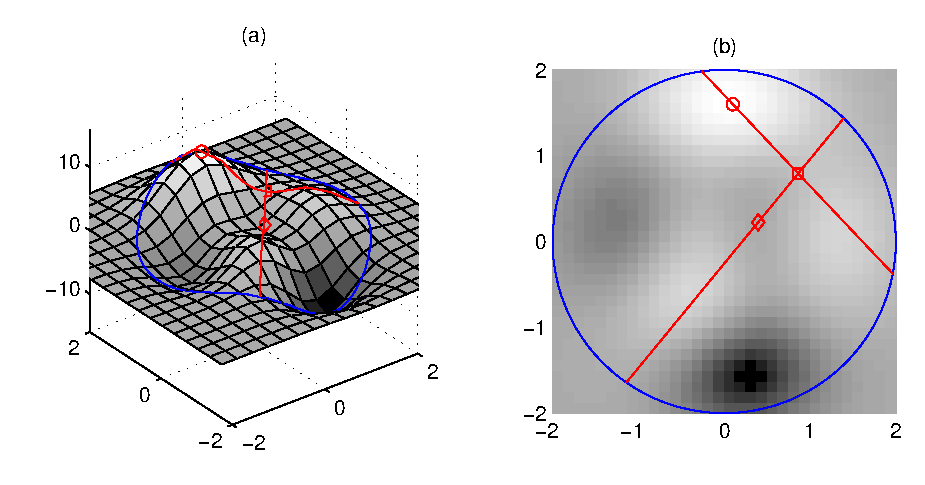
\includegraphics{figures/descent}
\end{center}
\begin{capt}{Schematic representation of gradient
descent.}{fig:gradient descent}
Points within the circle are in \calH, the height of the surface
the value of $C(\bfx)$ at that point.  (a) is a 3D view, (b) is plan
view. Lines show line searches; markers minima.  We descend from
$\circ$ through $\Box$ to $\Diamond$, where the algorithm terminates
due to a local minima.
\end{capt}
\end{linefigure}

We will now show that AdaBoost implements gradient descent using the
cost function $c(\lambda) = e^{-\lambda}$.  We do this by showing that
gradient descent produces the same $b_t$ and $\bfw_t$ values as
AdaBoost.

\begin{theorem}[AdaBoost implements gradient descent \cite{Mason99}]
\label{thm:adaboost gradient descent}
The AdaBoost algorithm implements gradient descent over a margin cost
function
%
\begin{equation}
\label{eqn:adaboost margin cost function}
c(\lambda) = e^{-\lambda}
\end{equation}
\end{theorem}

\proof We outline a skeleton, ignoring initial conditions and the
stopping conditions.  We will show that, given a state at iteration
$t$, then boosting and gradient descent produce identical states at
iteration $t+1$.

Once $\bbW$ has chosen $h_{t+1}$ using weighted empirical risk
minimisation, we choose $b_{t+1} = \alpha^{\ast}$ that minimises the
cost functional along the line $F_t + \alpha h_{t+1}$.  The value of
the cost functional along this line is
%
\begin{equation}
C = \sum_{i=1}^{m} c \left( y_i F_t(\bfx_i) + y_i \alpha
h_{t+1}(\bfx_i) \right)
\end{equation}
%
Substituting in (\ref{eqn:adaboost margin cost function}), we obtain
%
\begin{equation}
C = \sum_{i=1}^{m} \exp \left\{ y_i F_t(\bfx_i) + y_i \alpha
h_{t+1}(\bfx_i) \right\}
\label{eqn:cost functional along line}
\end{equation}
%
We minimise (\ref{eqn:cost functional along line}) by
differentiating with respect to $\alpha$ and setting the derivative to
zero.  The task is simplified considerably by noting that only the
second half of the exponential is a function of $\alpha$.  The result
is that
%
\begin{equation}
\label{eqn:differentiate}
\frac{\partial C}{\partial \alpha}
= \sum_{i=1}^{m} y_i h_{t+1}(\bfx_i) \exp \left\{ y_i F_t(\bfx_i) +
y_i \alpha h_{t+1}(\bfx_i) \right\} = 0
\end{equation}
%
We make several algebraic simplifications.  Noting that
%
\begin{equation}
y_i h_{t+1}(\bfx_i) = \left\{ 
	\begin{array}{rl}
	1 &	\qquad \mbox{if $y_i = h_{t+1}(\bfx_i)$} \\
	-1 &	\qquad \mbox{if $y_i \neq h_{t+1}(\bfx_i)$}
	\end{array}
\right. 
\end{equation}
%
and that $w_{t,i} = k \exp \{ -y_i F_t(\bfx_i) \}$ where $k$ is some
(normalising) constant, we recast (\ref{eqn:differentiate}) into
the form 
%
\begin{equation}
\overbrace{
\underbrace{
	\frac{\sum_{i : y_i = f_{t+1}(\bfx_i)} w_{t,i}}
	     {\sum_{i : y_i \neq f_{t+1}(\bfx_i)} w_{t,i}}
}_{\epsilon_t}
}^{1 - \epsilon_t}
= \exp \left\{ 2 \alpha^{\ast} \right\} 
\end{equation}
%
from which it is straightforward algebra to obtain $b_{t+1} =
\alpha^{\ast}$, the classifier weight
equation(\ref{eqn:theory:bt}). Thus, gradient descent updates the
internal state in the same manner as AdaBoost; therefore AdaBoost
implements gradient descent.

The cost functional $c(\lambda) = e^{-\lambda}$ is an approximation to
the misclassification risk (\ref{eqn:misclassification loss function})
that is differentiable at all points and leads to a closed-form
solution for the step size.  It is plotted in figure \ref{fig:cost
functional approximation}.  Other approximations have been used, a
survey of which appears in \cite{Mason99}.

\begin{linefigure}
\begin{center}
\includegraphics{figures/cost_approx}
\end{center}
\begin{capt}{Approximation to the misclassification risk
function}{fig:cost functional approximation}
The misclassification risk is plotted in the dotted line, with the
AdaBoost approximation plotted in the solid line.  It is clear that
the effect of this cost function will be to maximise the margins of
the samples.
\end{capt}
\end{linefigure}

\subsection{Modifying gradient descent}

We have shown that the AdaBoost algorithm implements gradient descent.
There are four degrees of freedom which can be exploited to produce
modified versions of gradient descent:
%
\begin{enumerate}
\item	Choice of universal set? (AdaBoost: $\co(\calH)$)
\item	Choice of inner product? (AdaBoost: equation (\ref{eqn:inner
	product definition}))
\item	Choice of cost function? (AdaBoost: $c(\alpha) =
	e^{-\alpha}$)
\item	Method of choosing step size? (AdaBoost: line search).
\end{enumerate}
%
In chapter \ref{chapter:pboosting} we consider alternative choices for
1, 3 and 4 to generate algorithms with desirable properties.


\section{AdaBoost and Boosting algorithms}

Until this point we have only considered the AdaBoost algorithm.  We
now extend our scope to other AdaBoost-like algorithms.  These
algorithms are termed ``boosting algorithms''.

There has recently been some debate over what constitutes a ``boosting
algorithm''; see for example Duffy and Helmbold \cite{Duffy99} who
adopt a quite restrictive definition.  In this thesis, we take a very
broad definition, allowing any learning machine that is operating in
an ``AdaBoost-like'' manner to be called a ``boosting'' algorithm.  In
particular, we don't require that the training error be guaranteed to
reach zero.


\section{Properties of AdaBoost}

We have covered the intrinsic properties of the AdaBoost algorithm quite
extensively.  We now cover some extrinsic properties, allowing
comparison of AdaBoost to other algorithms in chapter
\ref{chapter:results}.

\subsection{Convergence properties}

\begin{theorem}[AdaBoost converges to zero training error in finite
time \cite{Freund97}]
\label{thm:AdaBoost training error convergence}
Suppose that the AdaBoost algorithm $\bbB$ operating on weak-learning
algorithm $\bbW$ generates hypotheses $h_t$ with training errors
$\epsilon_1, \ldots, \epsilon_T$ over a training set $X$.  Furthermore,
assume that each $\epsilon_t < 1/2$, and let $\beta_t = 1/2 -
\epsilon_t$.  Then the empirical risk of the \emph{combined}
hypothesis $H_T = \sign(F_T)$ is bounded by
%
\begin{equation}
R_{\emp}(H_T) \leq \prod_{t=1}^{T} \sqrt{1 - 4 \beta_t^2} \leq \exp
\left\{ - 2 \sum_{t=1}^T \beta_T^2 \right\}
\end{equation}
\end{theorem}

\proof The straightforward proof of this theorem is contained in
\cite{Freund97}.\vspace{\baselineskip}

The following theorem shows that the total weight of the boosting
algorithm is unbounded as the number of iterations increases.  It is
used to prove results on the minimum margin and final training error
of boosting.

\begin{theorem}[Sum of AdaBoost classifier weights is unbounded]
\label{thm:classifier weights unbounded}
Suppose that we are given a set of training samples $X$ and a
weak-learner $\bbW$, and run AdaBoost for $T$ training
iterations.  Then either
%
\begin{itemize}
\item	AdaBoost terminates on an iteration $t_{\mathrm{term}} < T$;
	or
\item	the $1$-norm%
	\footnote{For a vector $\bfb \in \bbR^n$, $\|\bfb\|_p = \left
	( \sum_{i=1}^{n} b_i^p \right)^{\frac{1}{p}}$ and $\|\bfb\|_1
	= \sum_{i=1}^{n} b_i$.}
	of the classifier weight vector $\mathbf{b}$ is
	unbounded as $T \rightarrow \infty$:
	%
	\begin{equation}
	\lim_{T \rightarrow \infty} \| \mathbf{b} \|_1 = \infty
	\end{equation}
\end{itemize}
\end{theorem}

\proof This is proved in \cite{Breiman97}.  The proof proceeds by
contradiction, assuming a least upper bound on $\|\mathbf{b}\|_1$ and
showing that this bound will only hold if training terminates.


\subsection{AdaBoost maximises the minimum margin}

This section shows that the limiting behaviour of AdaBoost is to
choose the linear combination that maximises the minimum margin over
its training samples.

\begin{theorem}[AdaBoost maximises the minimum margin]
\label{thm:maximises minimum margin}
Given a particular hypothesis $F$ and a training set $X$, define the
minimum margin as 
\[
m_{\min} = \min_{(\bfx_i,y_i) \in X} y_i F(x_i)
\]
Then the AdaBoost algorithm will converge as $t \rightarrow \infty$ to
the solution which maximises the minimum margin.
\end{theorem}

\proof We present an outline (assuming that training doesn't
terminate).  We can write AdaBoost's hypothesis as $F_t = b_1 h_1 +
\cdots + b_t h_t$. Then defining the \emph{normalised hypotheses}
$\bar{f}_i$ as  
%
\begin{equation}
\bar{f}_i = \frac{b_i h_i}{\|b\|_1}
\end{equation}
%
such that $\bar{F}_t = \bar{f}_1 + \cdots + \bar{f}_t$, the cost
functional (\ref{eqn:cost functional along line}) can be rewritten as
%
\begin{equation}
\label{eqn:normalised cost}
C(F) = \sum_{i=1}^{m} \exp\{-y_i \bar{F}_t(\bfx_i)\}^{\|b\|_1}
\end{equation}
%
We know from theorem \ref{thm:adaboost gradient descent} that
AdaBoost is working to minimise the cost function.  From theorem
\ref{thm:classifier weights unbounded},  $\|b\| \rightarrow \infty$;
thus as $t \rightarrow \infty$ the largest value of $-y_i
\bar{F}_t(x_i)$ will dominate the sum (\ref{eqn:normalised cost}), and
so $C(F) \rightarrow exp\{\max -y_i \bar{F}_t(x_i)\}$.  Thus, to  
minimise $C(F)$ we must be making $\min y_i \bar{F}_t(x_i)$ as large
as possible; that is we are maximising the minimum margin.  Figure 
\ref{fig:adaboost margins} illustrates the evolution of both the cost
function and the margins of a dataset.

\begin{linefigure}
\begin{center}
\includegraphics{figures/adaboost_margins}
\end{center}
\begin{capt}{Cost function and margin evolution of
AdaBoost}{fig:adaboost margins}
Each curve was generated by training AdaBoost on a small dataset.  The
lines indicate a snapshot at a particular time: 5 iterations (solid),
50 iterations (dashed) and 1000 iterations(dotted).

Part (a) shows the \emph{normalised} cost function $c(\gamma) =
e^{-\|\mathbf{b}\| \gamma}$.  It is clear that as $t \rightarrow \infty$,
this cost function becomes very steep.  Part (b) shows a cumulative
distribution of the normalised margins (that is, the proportion of
samples with margin less than or equal to $\gamma$.  As time
progresses, the minimum margin is pushed further to the right; at 1000
iterations the training error has evidently reached zero as all
margins are positive.  (Note that for clarity part (b) has its $x$
axis normalised separately for each $p$ value in order to stretch the
margin distribution over the whole range.)
\end{capt}
\end{linefigure}


\subsection{Invariance of AdaBoost to uniform scaling of classifier
weights}

We present here an obvious theorem about the invariance of hypothesis
weights.  It has some implications on the hypothesis classes that the
$p$-boosting algorithms discussed in chapter \ref{chapter:pboosting}
use.

\begin{theorem}
\label{thm:invariance}
The hypothesis returned by the AdaBoost is independent of a 
scaling of the $b$ values.  Given an unthresholded hypothesis $F$ and
a constant $\alpha > 0$,
%
\begin{equation}
H = \sign(F) \equiv H' = \sign(\alpha F) 
\end{equation}
\end{theorem}

\proof This follows easily from the fact that the sign function is
unaffected by a constant scaling.



\section{Performance bounds for Boosting}

The following theorem appears in Schapire et. al \cite{Schapire97}.
It gives a bound on generalisation error similar to those in chapter
\ref{chapter:slt}.

\begin{theorem}[Performance bound for boosting ($p$=1)]

There is a constant $c$ such that a combined hypothesis $H = \sign(F)$
generated by the AdaBoost algorithm $\bbB$ from a base class $\calH$
with VC dimension $d$, with probability at least $1 - \delta$ over $m$
independent training samples has true risk bounded by 
\begin{equation}
R(H) \leq R_{\emp}^{\gamma}(F) + \sqrt{\frac{c}{m} \left[ \frac{d
\ln^2 (m/d)}{\gamma^2} + \ln(1/\delta) \right] }
\end{equation}
\end{theorem}


\section{Overfitting}
\label{sec:boost overfitting}

Initial experiments with AdaBoost indicated that the algorithm was
remarkably resistant to overfitting, despite the unlimited complexity
of the hypothesis space \cite{Freund96}.
However, further experiments \cite{Grove98, Bauer99} revealed that
training to $10^4$ to $10^6$ iterations, or adding label noise, would
often induce overfitting.  Figure \ref{fig:overfitting graphs} shows some
examples of the effect.  There have been several studies into the
characteristics of AdaBoost that lead to overfitting \cite{Schapire97,
Grove98, Ratsch98}.  A largely intuitive survey of the characteristics
of AdaBoost that lead to overfitting is presented here. 

\begin{linefigure}
\begin{center}
\includegraphics{figures/boost_overfitting}
\end{center}
\begin{capt}{Experimental results for Boosting showing
overfitting}{fig:overfitting graphs}
Three plots of test/training error vs iteration number for Boosting.
The dataset used was the ``ring'' distribution (see chapter
\ref{chapter:method}) with 50 samples.  Mild overfitting is visible on
the 20\% noise plot and becomes more pronounced as the level of noise
increases.  The solid curve is the test error (true risk); the dashed
curve the training error.
\end{capt}
\end{linefigure}

That overfitting occurs in AdaBoost is a consequence of the property
that AdaBoost maximises the minimum margin (theorem
\ref{thm:maximises minimum margin}).  Intuitively, this property
causes the  AdaBoost algorithm to concentrate on a few hard
samples.  Unfortunately, in a noisy dataset, these samples are usually
all noise.  Some algorithms are mentioned in the next section that
explicitly allow for some samples to be misclassified, in order to
reduce the tendency towards overfitting.

\section{Previous work on regularising AdaBoost}

Following the discovery that AdaBoost operated by maximising the
minimum margin, several efforts were made to regularise AdaBoost to
avoid overfitting.  Algorithms such as \emph{soft margins}
\cite{Ratsch98} explicitly allow a certain number of training samples
to have a small or negative margin; while algorithms such as DOOM and
DOOM II \cite{Mason99a, Mason99b} do this implicitly by flattening out
the cost function (figure \ref{fig:cost functional approximation}) for
low and negative margins.  These approaches have been quite
successful, both outperforming AdaBoost under some conditions (in
particular on noisy data).


\section{Normed boosting algorithms}

Several authors \cite{Mason99a, Breiman97} have studied modified
versions of AdaBoost, where the classifier weights are
normalised \emph{at each iteration}.  After $b_t$ is calculated for
iteration $t$, the entire set of classifier weights $b$ are
normalised:
%
\begin{equation}
b_{i} \Leftarrow \frac{b_i}{\| \mathbf{b} \|_p} \qquad  i=1
\ldots t
\end{equation}
%
where the norm is chosen via the $p$ parameter.%
\footnote{Mason et. al. considered mainly $p \in \{ 1,2 \}$ in
\cite{Mason99a}.}

While it can be shown that these algorithms converge to the global
minimum of the gradient descent cost functional (\ref{eqn:gradient
descent cost functional}), they do \emph{not} have the property of
guaranteed convergence to zero training error (theorem
\ref{thm:AdaBoost training error convergence} does not hold); the
reason being that  $\sum_{i=1}^t b_{t,i}$ is bounded above (theorem
\ref{thm:classifier weights unbounded} does not hold).  As results in
chapter \ref{chapter:results} and the discussion in section
\ref{sec:boost overfitting} indicate, an algorithm does not have to
converge to zero training error to generalise well.

The ``sloppy'' algorithm developed in chapter \ref{chapter:pboosting}
is a generalisation of the normed boosting algorithm described in this
section, where the value of $p$ is any positive real.





